\documentclass[a4paper,notitlepage]{article}

\usepackage[english]{babel}
\usepackage{verbatim}
\usepackage{amsmath}
\usepackage{amssymb}
\usepackage{graphicx}
\usepackage{epstopdf}
\usepackage{supertabular}
\title{Arakoon manifesto}
\author{Romain Slootmaekers}
\date{July 2010}
\begin{document}

\maketitle
\abstract{
 Arakoon tries to be a simple distributed key value store 
 that prefers consistency above everything else.
}

%\tableofcontents
\section{introduction}
\subsection{What kind of document is this?}
This document was written mainly before we started building Arakoon. 
It served the purpose as a basis of discussion, 
trying to get consensus on what we were going to build, before we build it. 
We regularly come back to this document to record decisions, and to keep it anchored to reality. Currently, it's not very well structured, the focus being on \emph{getting the information in there first}. 
Hopefully there will eventually be time to clean it up.
\subsection{why Arakoon?}
We have been using several distributed non relational data stores for a long time now, and it has not been a satisfying experience.
\subsection{what we aim for}
We want a simple distributed key/value store that is easy to understand and use.
We don't need infinite scalability (and in fact we have several limitations), but we do have some requests regarding
\paragraph{consistency}
The system as a whole needs to provide a consistent view on the distributed state.
This stems from the experience that eventual consistency is too heavy a burden for a user application to manage. 
A simple example is a retrieval of the value for a key where you might receive none, one or multiple values depending on the weather conditions. The next question is always: Why don't a get a result? Is it because there is no value, or merely because I currently cannot retreive it?

\paragraph{conditional atomic updates}
We don't need full blown transactions (would be nice to have though), 
but we do need updates that abort if the state is not what we expect it to be.
So at least an atomic conditional update and an atomic multi-update are needed.
\paragraph{robustness}
The system must be able to cope with failure of individual components, without concessions to consistency.
However, whenever consistency can no longer be guaranteed, updates must simply fail.
\paragraph{locality control}
When we deploy a system over 2 datacenters, we want guarantees that the entire state is indeed present in both datacenters. (This is something we could not get from distributed hash tables using consistent hashing)

\paragraph{healing/recovery}
Whenever a component dies and is subsequently revived, or replaced the system must be able to guide that component towards a situation where that node again fully participates. 
If this cannot be done fully automatically, then human intervention should be trivial.
\paragraph{explicit failure}
Whenever there is something wrong, failure should propagate quite quickly.
This in contrast to systems that keep on trying to remedy the situation themselves al the time.
\subsection{Isn't this what Keyspace does?}
Almost. We used keyspace for a while but were struggling with some issues.

\paragraph{atomic multi updates}
With Keyspace, you can do multiple updates in one request, 
but it's nowhere near atomic, so when one of them fails, you're in limbo. Arakoon supports a sequence update which is an all or nothing thing.
\paragraph{test\_and\_set}
This is a conditional update, that only changes a value for a key when the store has the expected state.
Keyspace supports this, but not when there is no expected value. 
This makes it impossible to atomically set a value only if it was not present.
An Arakoon \emph{test\_and\_set} can be used to set a new value, 
update an existing value, or remove an existing value.
It's also important to notice Arakoon returns the \emph{old} value after a
\emph{test\_and\_set}, allowing one to determine whether an update took place
\paragraph{Keyspace defects}
\begin{itemize}

\item{} Segmentation violations under heavy load.
\item{} Accidental semantic changes of the interfaces
\item{} Keyspace nodes happily accept data even when the disk is full.
\item{} Several cluster in limbo (no updates possible) scenarios.
\item{} abandoned python client. There used to be a pure python client, 
but now it's abandoned in favour of a \emph{SWIGed around C} library, 
which enforces it's own reconnection strategy.
\item{} Berkeley DB.\footnote{May, 2011, Scalien dropped Keyspace due to \emph{'BerkeleyDB issues'}} 

\end{itemize}
It's not that these issues are impossible to address. It's just that when you're fighting these, you don't want to be owner of the problem, not a spectator.
\subsection{high level overview}
Arakoon deployments consist of a small collection of \emph{nodes} (typically 1,2,3 or 5 nodes) that keep replicas of key/values, and \emph{clients} that manipulate the key/value space.
In principle, all nodes have the entire key/value space.
There is one distinguished node called the master with which all clients communicate to perform updates.
A client contacts any node to find out the master, and then just conversates with the master.
If a master dies, a new one is elected automatically, and clients fail over to that master.
A slave node is a node that is not master.
A node that is not up-to-date cannot become master.

\subsection{limitations}
\paragraph{capacity}
Since all nodes store the entire space, the capacity of the smallest node limits the system.
\paragraph{number of clients}
Since all updates go through the master, the system is not suited for large amounts of concurrent clients.
\paragraph{opaque values}
The system does not really understand the values, and hence cannot do validation, or transformations \ldots
\paragraph{hidden master failure}
If the key value store on the master silently corrupts, gets will be affected.


\section{basic client interface}
\subsection{some notation}
Before we can descibe the client's interface, 
we need to introduce some notational tools to make it easier to convey things in a concise manner.

\begin{table}[h]
\begin{tabular}{|l|l|}
\hline
  notation & how to read it \\
\hline
  :                & has type \\
unit               & aka void  \\
x list             & a list of items of type x \\
x array            & a fixed size sequence of items of type x \\
x option           & either (Some x) or None \\
string             & char array \\

$ x \rightarrow y$ & a function from x to y \\
x C.t              & something that \emph{eventually yields} something of type x \\
\hline
\end{tabular}
\end{table}

For example $ a : string $ just means that $a$ is a $string$;
$fibonacci : int \rightarrow int$ just means that fibonnacci is a function that takes an integer, and returns an integer as result;
$cat : string \rightarrow string \rightarrow string$ reads as 'cat is a function that takes 2 strings and returns a string as result'

$write: channel \rightarrow string \rightarrow unit\ C.t$ reads as 'write takes a channel and a string and eventually yields unit.


A client has a dictionary interface with some adjustments for latency: the functions have a return value of type $a\ C.t$.
\paragraph{type key = string}
Keys are strings.
There are no strict size limitations, which means that they such be small enough to be handled in their entirety
\paragraph{type value = string}
Values are strings too.
\paragraph{type update}
An update is either $Set(key,value)$ or $Delete(key)$.
\paragraph{exists : key $\rightarrow$ bool C.t} See if a value exists for a specific key, without retrieving it.
\paragraph{get : key $\rightarrow$ value C.t}
You can look up a value if you have the key. It will eventually yield either a value, or raise an exception.
\paragraph{set : key $\rightarrow$ value $\rightarrow$ unit C.t}
You can update a value for a key, regardless of current value (if any).
\paragraph{delete : key $\rightarrow$ unit C.t}
You can remove a key/value pair. 
There was a suggestion to open this op to allow a regular expression.

\paragraph{test\_and\_set : key $\rightarrow$ value option $\rightarrow$ value option $\rightarrow$ (value option) C.t} This is a careful update.
\emph{test\_and\_set k expected new} only modifies the value to \emph{new} if the old value is \emph{expected}.
The originaly stored value will be returned.
Using a \emph{value option} instead of a value allows you to only set a value only if there was none for that key.
Using \emph{None} as new allows you to do a careful delete as well.

\paragraph{range : key option $\rightarrow$ bool $\rightarrow$
  key option $\rightarrow$ bool $\rightarrow$
  int $\rightarrow$ key list C.t}
\emph{range bkey binc ekey einc max} will yield a list of keys where
$max$ is the maximum number of keys (if $max < 0$ then you want them all).
The keys fall in the range \emph{kbey..ekey}.
\emph{binc} and \emph{einc} specify if the borders are included (\emph{true}) or not.
\paragraph{range\_entries: key option $\rightarrow$ bool $\rightarrow$
  key option $\rightarrow$ bool $\rightarrow$
  int $\rightarrow$ bool $\rightarrow$ (key * value) list C.t
}
will yield a list of key value pairs.
The parameters have the same semantics as for the range method.

\paragraph{sequence: update list $\rightarrow$ unit C.t}
Provides an atomic multi-update. Either all updates are performed or none. 
While this is not a full transaction, it provides enough functionality to safeguard consistency.

%\paragraph{hello : string $\rightarrow$ string $\rightarrow$ string C.t}
%The client identifies itself to the server and tells the server the cluster id, and the server replies with its version string.

\paragraph{who\_master: unit $\rightarrow$ string option C.t}
Allows the client to know which node currently acts as master.
If there is no master, or it is not known to this node, the result is None.
%
%\paragraph{last\_entries: int $\rightarrow$ out\_channel $\rightarrow$ unit C.t}
%allows the client to stream the transaction log into a channel, starting from entry $i$

\paragraph{multi\_get: key list $\rightarrow$ (value list) C.t}
Allows you to fetch multiple values in one roundtrip to the server.

\paragraph{expect\_progress\_possible: unit $\rightarrow$ bool C.t}
Asks the master node if it thinks progress is possible. 
This means that the master has seen enough that indicates enough slaves are still following its lead. 
False positives are possible.


\section{Consistent updates}
An update is sent to the master.
The master adds it to its log, and tries to get consensus about the update with the slaves.
Once consensus has been reached about the first log entry,
the master adds the entry to the persistent local key-value store.
Slaves can move the updates from their log
into their local key-value store asynchronously.

\begin{figure}
\begin{verbatim}
(nicked from wikipedia)

C      M            S0  S1
|      |            |    |  --- first request ---
X----->|            |    |  Request
|      X----------->|--->|  Prepare(N)
|      |<-----------X----X  Promise(N,  I, {Va,Vb,Vc})
|      X----------->|--->|  Accept!(N,  I, Vn)
|      |<-----------X----X  Accepted(N, I)
|<-----X                    Response
                            --- other requests ---
X----->|            |    |  Request
|      X----------->|--->|  Accept(N,   I+1, W)
|      |<-----------X----X  Accepted(N, I+1)
|<-----X            |    |  Response

X----->|            |    |
|      X----------->|--->|  Accept(N, I+2,  X)
|      |<-----------X----X  Accepted(N,I+2)
...
\end{verbatim}
\end{figure}
The first request with M as Master (= leader) needs a full paxos round,
while subsequent updates with the same leader skip the first phase.
This boils down to a single roundtrip from master to slaves per update.
If the different nodes have failure modes independent of each other (independent power supplies, different disks, \ldots),
one needs not await the push-through to disk and the message can be pushed asynchronously to the local key-value store.
This optimistic behaviour needs to be a configuration option, since the application cannot assess this by itself.
One can also go below 1 roundtrip per update by stuffing multiple updates together.
This increases throughput.


\subsection{Individual Slave failure}
If a slave dies, the master is not affected.
When a slave comes up, there are three possibilities. 
The first is not very interesting. If the slave's log matches that of the master, nothing happened meanwhile and the slave is \emph{in sync}. 
The other cases are \emph{small lapse} and \emph{big lapse}.
\paragraph{small lapse}
Its replication counter I is still within the log of the master
(or other any other slave that has a more recent state) . 
So the slave first downloads the missing part of the log.
Then it iterates over the tlog while adding the missing updates to the store.
When finished the client again compares its log state with that of the other nodes. 
It's either in back in sync or again within in a small lapse. 
When the master is under load, it can be that a slave loops here until the master slows down.

\paragraph{big lapse}
Small lapse would be enough if one keeps the log files. 
The only problem with this is that it wastes more than half of the available diskspace. 
The good news is that these log files compress quite well, 
so the only thing we want to be able to do is compress log files when rotate, 
and make sure we can still read the compressed logs. 
We also plan to implement the \emph{collapsing} of logs: 
Several updates for the same key can be replaced with the last update under certain conditions.
Applications that only manage a limited set of keys, but update the values frequently will benefit from this a lot.
\section{Electing a master}
Master election should happen using paxos. 
A master choice has a timeout, and a master tries to relect itself before the lease expires.
Details are described in the PaxosLease paper.


\section{Restart and Failure Scenarios}
Comprehension greatly benefits from writing out explicitly what should happen after a failure\footnote{Something we learned the hard way}.

\subsection{General power failure, after which the master is dead meat}
\tablehead{
  \multicolumn{2}{|c|}{A}& 
  \multicolumn{2}{|c|}{B}&
  \multicolumn{2}{|c|}{C}
  \\\hline}
\begin{supertabular}{|cl|cl|cl|}
  000 & $^s$MasterSet('C',\ldots) & 000 & $^s$MasterSet('C',\ldots) & 000 & MasterSet('C',\ldots) \\
  001 & $^t$Set('x','X')          & 001 & $^t$Set('x','X')          & 001 & $^{s,t}$Set('x','X')   \\
\hline
\end{supertabular}
\paragraph{}
The table shows the situation when the power goes off. 
Node C became master and dictated 1 update (\emph{Set('x','X')}), received \emph{Accepted} messages from all slaves,
after which it pushed that update to its store. 
The question is, what happens when node C is lost and A and B are started again?

\paragraph{}
It's obvious that globally, there should be consensus on the \emph{Set} update, but since there was no follow up, 
both nodes don't realise this yet, and are trying to find out what should happen.
A sends out a \emph{Prepare(n,i=1)} to which B answers with a \emph{Promise(n,i=1,Set('x','X'))}.
All goes well, and A receives the promise, and thus decides that this is indeed the value for \emph{i=1}.
It pushes the value, to the store. 
Node A goes into a state identical to C, before it became defunct.
\paragraph{}
If node A gets this far, it's a de-facto leader, and can start acting like it. 
The next thing A does is broadcast \emph{Accept(n,2,MasterSet('A',\ldots)} and things will soon be normal again.

\subsection{Unfortunate sequence of events}
\tablehead{
  \multicolumn{2}{|c|}{N1}& 
  \multicolumn{2}{|c|}{N2}&
  \multicolumn{2}{|c|}{N3}
  \\\hline}
\begin{supertabular}{|l|l|l|l|l|l|}
  i-1 & $^s$v0 & i-1 & $^t$v0 & i-1 & $^t$v0\\\hline
  i   & $^t$v1 &   i &        &   i &       \\
\hline
\end{supertabular}
\paragraph{}
A the starting situation is reached by a cluster where N1, being master accepted \emph{v1} at \emph{i} after which aferything goes down.
After this, there are some problems with the master node (N1) and only N2 and N3 are restarted.
They come up, resume service, and accept and reach consensus on a new value \emph{v2}.
\\
\tablehead{
  \multicolumn{2}{|c|}{N1}& 
  \multicolumn{2}{|c|}{N2}&
  \multicolumn{2}{|c|}{N3}
  \\\hline}
\begin{supertabular}{|l|l|l|l|l|l|}
  i-1 & $^s$v0 & i-1 & $^s$v0 & i-1 & $^s$v0\\\hline
  i   & $^t$v1 &   i & $^t$v2 &   i & $^t$v2\\
\hline
\end{supertabular}
\paragraph{}
Then, disaster strikes again, and both N2 and N3 are stopped. 
There seems to be a problem with N3, but the sysads did a great job and restored N1.
Both N1 and N2 are started. 
Now N1 promises v1 to N2 and N2 promises v2 to N1. 
Neither can reach consensus and progress is blocked.




\section{Implementation choices}
\subsection{Inter-node communication}
The nodes are fully connected with each other over tcp sockets.
The low level (de-)serialization is handled by our llio library (C,Python and ocaml implementations available).
This library is actually pretty efficient.
For example, on inteloids, fetching a 64 bit integer from a buffer boils down to a reinterpretation of 8 bytes in the buffer (in C, it merely is a cast, while in Python it's a \emph{struct.unpack('q',i)} ).
Nodes all know one another from their configuration.
Just above the socket layer, there's an abstract messaging layer, where you can just send and receive messages.



\subsection{Client-Node communication}
The client node communication has different needs, and hence a rpc like approach will be used. Following table describes what we do with primitives.
Just note that a list should be written out head first, so that naieve de-serialization will return the original.
\begin{table}[ht]
\begin{tabular}{lll}
type  &   marshalled form & size (bytes)          \\
\hline
bool        & false $\rightarrow 0 | $ true $ \rightarrow 1   $ & 1 \\
int32       & big endian          & 4             \\
int64       & big endian          & 8             \\
string      & [size:$int_{32}$][bytes] & 4 + n     \\
float       & IEE754 double       & 8             \\
x option    & 0x00 (None) or 0x01 [x] & $|x| + 1$ \\
x list      & [size:$int_{32}$][$x_{n-1}$]\ldots[$x_{0}$] \\
x array     & [size:$int_{32}$][$x_{0}$]\ldots[$x_{n-1}$] \\
\hline \\
Set(key,value) & [1:$int_{32}$][key:string][value:string]\\
Delete(key) & [2:$int_{32}$][key:string]\\
sequence    & [size(data):$int_{32}$][$bytes(data)$] \\
\hline
\end{tabular}
\end{table}

\subsubsection{protocol definition}
The protocol is a very simple request/response based binary protocol.
The client is the active party, and sends a command
\paragraph{successful rpc call}
\begin{equation*}
\begin{aligned}
client: \ & [command:int_{32}][parameter_0][parameter_1]\ldots & (\&flush) \\
server: \ & [0x0:int_{32}][result_0][result_1]\ldots & (\&flush)
\end{aligned}
\end{equation*}
\paragraph{call that failed}

\begin{equation*}
\begin{aligned}
client: \ & [command : int_{32}][parameter_0][parameter_1]\ldots & (\&flush) \\
server: \ & [rc:int_{32}][size:int_{32}][bytes] & (\&flush) \\
\end{aligned}
\end{equation*}

Each command is masked with the magic sequence $0xb1ff0000$.
The node checks the magic, proceeds with reading the parameters, and processes the request.
Then the response code and response are written.
If a failure happens, the server writes out a return code different from zero, and a string with a message after which he closes the connection.

The command codes and return codes are listed below.
The first thing a client does after establishing a connection is a \emph{hello} call so that the server can identify the client (handy for logging, etc).
\begin{table}[ht]
\begin{tabular}{ll}
return code & condition \\
\hline
0x0000 0000  & success!  \\
0x0000 0001  & command has no magic  \\
0x0000 0002  & too many dead nodes \\
0x0000 0003  & no hello        \\
0x0000 0004  & not master      \\
0x0000 0005  & not found       \\
\ldots       & \ldots          \\
0x0000 00ff  & unknown failure \\
\end{tabular}
\end{table}

\begin{table}[ht]
\begin{tabular}{ll}
command & code \\
\hline
hello          & 0x0000 0001 \\
who\_master    & 0x0000 0002 \\
exists         & 0x0000 0007 \\
get            & 0x0000 0008 \\
set            & 0x0000 0009 \\
delete         & 0x0000 000a \\
range          & 0x0000 000b \\
prefix\_keys   & 0x0000 000c \\
test\_and\_set & 0x0000 000d \\
last\_entries  & 0x0000 000e \\
range\_enties  & 0x0000 000f \\
sequence       & 0x0000 0010 \\
multi\_get     & 0x0000 0011 \\
expect\_progress\_possible & 0x0000 0012 \\
\hline
\end{tabular}
\end{table}

\subsection{nodes in ocaml}
Implementing the nodes in ocaml using Ocsigen's LWT library gives ample control over the fine grained concurrency we need through monadic coroutines.
\subsection{Pure Python client}
Besides the obvious ocaml client, Arakoon provides a pure python client as well. We have other in house projects that need it.

\subsection{other clients}
We've more or less catered for our own needs (Python,ocaml and C).
Other clients will have to implement our client-node protocol. 
Meanwhile, someone wrote an experimental Erlang client in less than a day's work. We're starting to run into problems because we have to maintain 3 clients instead of one.

\subsection{local key/value store}
We've picked tokyo cabinet. 
Our client interface matches its api quite well. 
It might be an idea to make this pluggable, but we don't need this at the moment.
Tokyo Cabinet is great for small values, but it will not cope with values of 1MB; 
even 10KB gives problems if you don't tweak the parameters. 
In essence, allowing both 1B and 1MB in the same BTree will eventually explode.

\subsection{forced master and quorum}
We needed to solve the case where you have only 2 nodes.
The simplest solution is to allow the master to be chosen by configuration and the quorum to be fixed. 
This way, you can chose for the 2 node case where you want the master, 
and if you're willing to take the risk to keep on writing in a case of a slave node not responding, you just set the quorum to 1.

\section{Other strategical decisions}
\subsection{REST interface}
We decided not to offer a REST interface.
\subsection{dynamically adding nodes}
All the nodes know one another from their configuration files,
but adding a node is not trivial. 
For example, one wants to add a third node in a two node setup and starts a node with a config referring to the two existing nodes. 
But these older nodes are clueless 
and have another opinion on how many nodes need to concur. 
A cluster protects itself by not answering to nodes it does not know; 
but this means adding a node means you need to restart the existing nodes.

\paragraph{}
It might be better to make the \emph{known\_nodes} a paxos value 
over which consensus must be reached, but this has additional risks.
The population can only change with reasonable increments.


\section{State machine}

\begin{figure}[ht]\label{fig:paxos}
  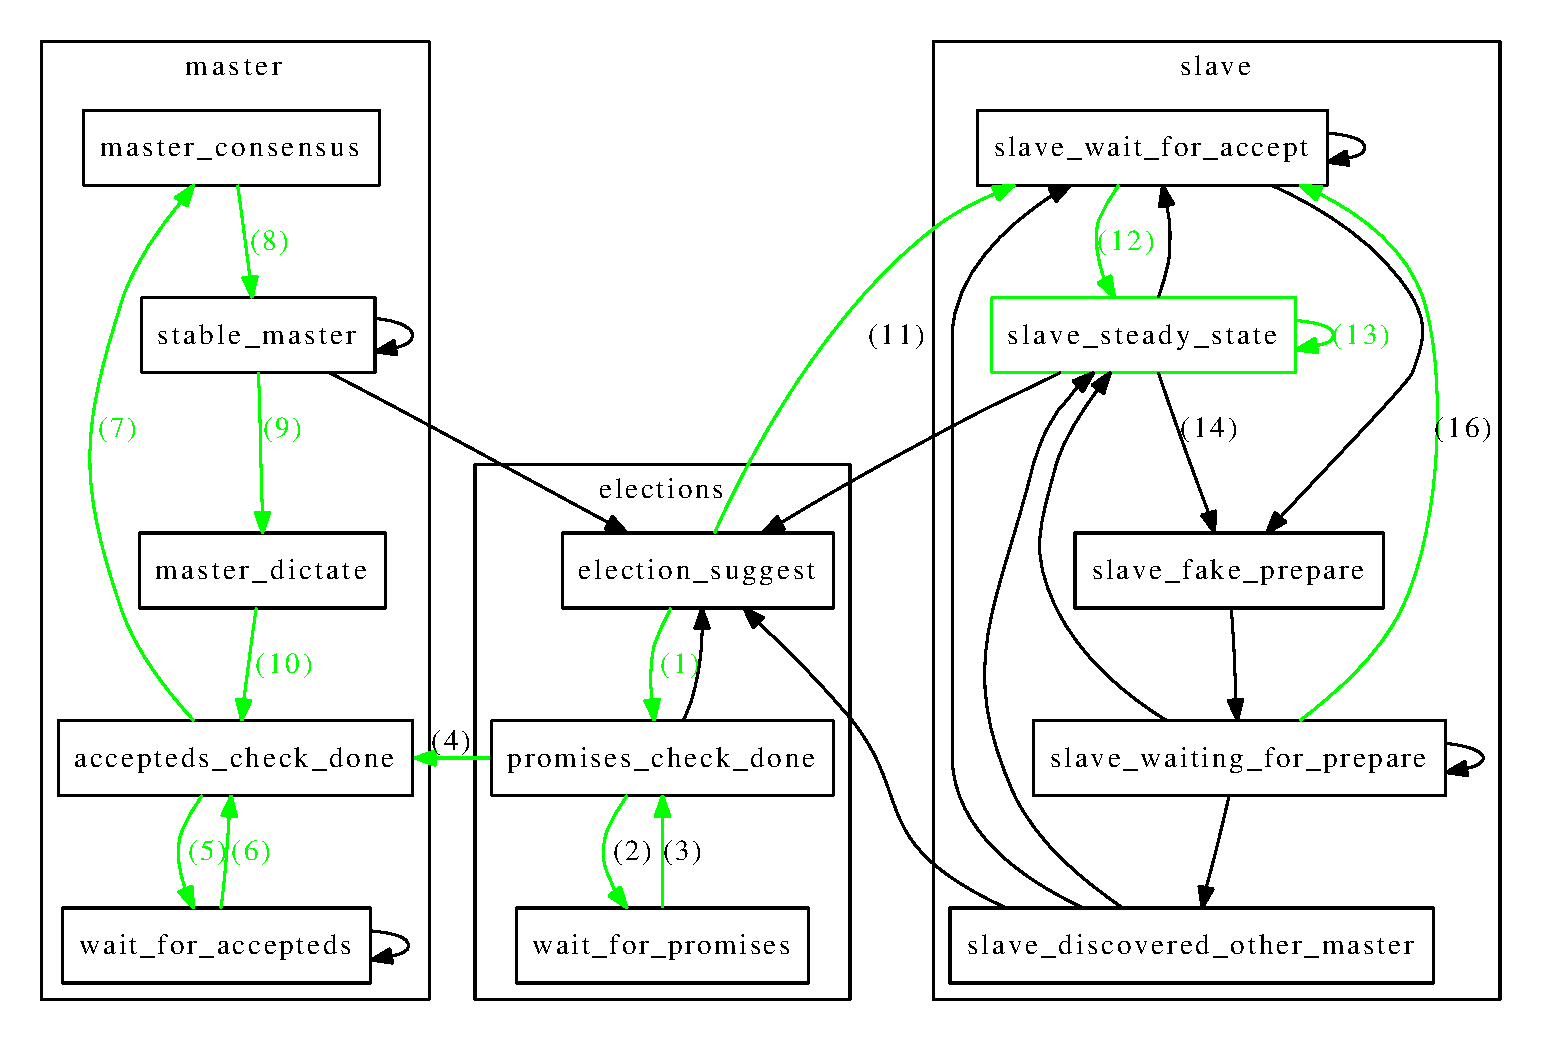
\includegraphics[width=\textwidth]{doc/states.eps}
  \caption{multi paxos state machine}
\end{figure}
Figure \ref{fig:paxos} shows the state machine diagram for the arakoon nodes. 
\begin{table}
\begin{tabular}{ll}
1  & /multicast Prepare n' \\
2  & to\_receive $>$ 0/ \\
3  & Promise(n,$new_i$,limit)/ \\
4  & to\_receive $=$ 0/ multicast Accept(n,$new_i$,v)\\
5  & needed $>$ 0/\\
6  & Accept(n,i)/\\
7  & needed $=$ 0/\\
8  & /start lease\\
9  & FromClient / \\
10 & multicast Accept(n,i,v) \\
11 & Prepare(n'>n)\\
12 & Accept(n,i,v)\\
13 & Accept(n,i,v)\\
14 & Accept(n',i',v')\\
15 & /multicast Prepare(-1)\\
16 & Prepare(n)/\\
\end{tabular}
\end{table}

\section{Scaling Arakoon}
We want to be able to use arakoon for increasingly large key-value spaces. 
For a single arakoon cluster the capacity is limited by the size of a single disk. 
So it is only natural to allow different arakoon clusters to team up. 
A \emph{nursery}\footnote{after a \emph{a nursery of raccoons}} provides a semi-unified view on a set of arakoon clusters. 
Each cluster is uniquely responsible for a prefix range. 
\subsection{Limitations}
The simple strategy of mapping a cluster to a range of keys already implies some limitations compared to the single cluster setup. 
As a result, applications willing to scale from a single cluster to a nursery need to do some planning.
\subsubsection{impact on sequences}
Sequences are multiple updates that are done atomically. 
Since atomicity can only be achieved inside 1 cluster\footnote{you could build transactionality across clusters, but it's a can of worms}, this means that all keys for a sequence need to share the same prefix. 
\subsubsection{impact on ranges}
Every cluster is responsible for a specific range. 
As client range query will only be served by a single cluster, it means that only ranges that are subranges of cluster ranges can be served.
\subsection{Migrations}
Once a cluster is filled, one needs to be able to split it, or move part of its range elsewhere. This process is called migration.
Each cluster has a \emph{public} range $[k_b,k_e)$ it serves to clients, as well as a \emph{private} range it contains. 
As such, migrating a part of a cluster's range to another cluster becomes feasible. 
If we're moving keys away from a \emph{source} cluster $[k_b, k_e)$ 
to a \emph{target} cluster $[k_e, k_z)$, we
\begin{itemize}
\item{} shrink the public range of the source cluster from 
$[k_b, k_e)$ to $[k_b, k_e - a)$. 
The private range of the source remains $[k_b, k_e)$
\item{} add the key/value pairs in $[k_e - a,k_e)$ to the target cluster
\item{} extend the public range of the target cluster from
$[k_e,k_z)$ to $[k_e - a, k_z)$
\item{} delete the key/value pairs on the source in $[k_e -a,k_e)$.
        update the private range on the source to $[k_b, k_e-a)$.
\end{itemize}
This work can be done by a privileged client responsible for the migration. 
That client can die at any point, and figure out, at resumption, what it needs to do to complete the task. 
The problem with the migration strategy is that there is a point in time where none of the clusters is serving $[k_e -a, k_e)$, so any request for anything in that range is refused.

\subsection{Client side support}
Each client needs to know which cluster is responsible for a certain key(-range). 
This information is kept in a routing table. At construction time, a client fetches this from a designated Arakoon that knows all the clusters in a nursery. 
The privileged clients performing migrations also must update this designated arakoon. 
As far as clients are concerned, it's not really important that the nursery clients have correct routing tables: 
If a client asks something from a cluster that's not able to comply, it will simply refuse. 
This means that either, there is some migration, or that the client has outdated routing information. 
In that case, it can simply refetch the ranges from the clusters it knows, or refetch it from the designated arakoon that keeps this information.
\subsection{Problems}
We depend on having a designated arakoon that knows all the clusters in a nursery, and their routing tables. 
So conceptually, we introduced a single point of failure. 
Since this point is in reality an arakoon cluster which is synchronuously replicated, that should not pose big practical problems.
\paragraph{}
Having to maintain configuration of (multiple/many?) arakoon clusters on lots of machines will become a significant problem. 
As this information is both crucial, and maintained by humans, which is a recipe for disaster. In time, we should move to service discovery. 
Possible options are:
\begin{itemize}
  \item{XMPP disco}
  \item{DNS-Based Service Discovery}
  \item{openSLP}
  \item{Salutation}
  \item{UPnP}
  \item{svrloc}
  \item{\ldots}
\end{itemize}



\end{document}
